
\documentclass[11pt]{article}

\usepackage{graphicx}			
\usepackage{tikz}
\graphicspath{ {../Figures/} }
\usepackage{amsmath}
\usepackage{mathtools}
\usepackage{amssymb, amsthm}
\usepackage{xcolor}
\usepackage{hyperref}
\usepackage{parskip}
\usepackage{scrextend} 
\usepackage{empheq}
%\usepackage[most]{tcolorbox}
%\usepackage[absolute,overlay]{textpos}

\newcommand{\braket}[2]{\textsf{\big{<}} #1 \textsf{\big{|\,}} #2\textsf{\big{>}}}
\newcommand{\ketbra}[2]{\textsf{\big{|}} #1 \textsf{\big{>}}\textsf{\big{<}} #2\textsf{\big{|}}}

\usepackage[matrix,frame,arrow]{xypic}
\usepackage[braket,qm]{qcircuit}


\begin{document}
	
	\title{Quantum Machine Learning: Variational Quantum Classifier}
	\author{Noah Hamilton}
	\date{\today}
	
	\maketitle
	\tableofcontents

\newpage
\section{What is Quantum Machine Learning?}\label{intro}

Quantum Machine Learning (QML) is a cross-section between Quantum Computing and Classical Machine Learning. 
Quantum Computing takes advantage of quantum mechanics to provide an advantage in time and 
cost over classical computers~\cite{garcía2022systematic}. Machine Learning is a subset of the classical field known
 as Artificial Intelligence that focuses on using data and algorithms to imitate how humans learn~\cite{IBM}.
 This crossover between Quantum Computing and Machine Learning is being actively researched~\cite{garcía2022systematic}.
 
 The interplay between Quantum and Classical is usually classified in two ways: what is the input data (Classical or Quantum)
 and what is the computing platform (Classical or Quantum). Decades of research in machine learning typically falls into the
 category of Classical Computing with Classical Data. Recent research efforts have been trying to take advantage of 
 near-term quantum devices with classical data falling into the paradigm of Quantum Computing with Classical Data.

 This research effort focuses specifically on a method in Quantum Machine Learning known as Variational Quantum Classifier (VQC).
 The main task of a VQC is to train a quantum circuit on labelled samples to predict labels for new data.
 A VQC embeds classical data into a quantum circuit, applies a parameterized model, produces a measurement of the circuit to
extract labels, and updates the model using optimization techniques~\cite{BuildingAVQC}. This research implements a VQC on three
datasets and compares performance across different quantum models using Qiskit and scikit-learn. 

To fully understand the context of a VQC, it is important to grasp the classical machine learning classification problem.
This research will also use a known good classical machine learning technique known as Support Vector Machine (SVM) as a baseline
for performance comparison.

\section{Background: Classical Machine Learning}\label{bg_svm}

There are several types of machine learning: supervised learning, unsupervised learning, semi-supervised learning,
reinforcement learning, and deep learning~\cite{ucberkeley}. For the sake of brevity, this paper will focus on the concept
of supervised learning, which is requires the data to be pre-labeled so that the algorithm can see how accurate its
performance is~\cite{ucberkeley}.

 UC Berkeley School of Information describes supervised learning in three steps~\cite{ucberkeley}:
 \begin{enumerate}
    \item \textbf{A Decision Process:} A way to compute a prediction from a given input. 
    \item \textbf{An Error Function:} A way to check if the prediction is correct, and quantify how accurate it is.
    \item \textbf{An Optimization Process:} A way to change the decision process to give better predictions.
 \end{enumerate}

The classification problem falls into this supervised learning paradigm where labelled data is used to train a classical model 
and used to predict new samples. The problem can take the form of binary classification or multi-class classification. A binary
classification problem could be like distinguishing between cats and dogs, while a multi-class classification could be distinguishing
between different types of flowers.

A well-known application of this problem is used for Optical Character Recognition, where
a number/letter is hand-drawn and a computer attempts to guess which number/letter it is. More complicated applications of this
classification problem can be used in RF Machine Learning which takes RF Data in the form of spectrograms (Power vs. Frequency)
and attempts to predict the different types of modulation. All of these examples take lots of labelled input data, make a prediction, 
and then optimize based on the accuracy of the prediction. The formal definition of the classification problem can be found within 
the paper by Havlicek and others~\cite{Havl_ek_2019}.

One of the more popular and successful algorithms is known as \textit{Support Vector Machine} (SVM). The objective of SVM is use a 
linear decision boundaries to make predictions about the data. This solution is ideal for data that is linearly separable.

In Figure~\ref{fig:svm-classical}, an example SVM is used on the first two features in the Iris dataset~\cite{sklearnsvm}~\cite{sklearndata}.
This research uses a very simple SVM for comparison and benchmarking in an image classification task.
\begin{figure}[!h]
    \centering
    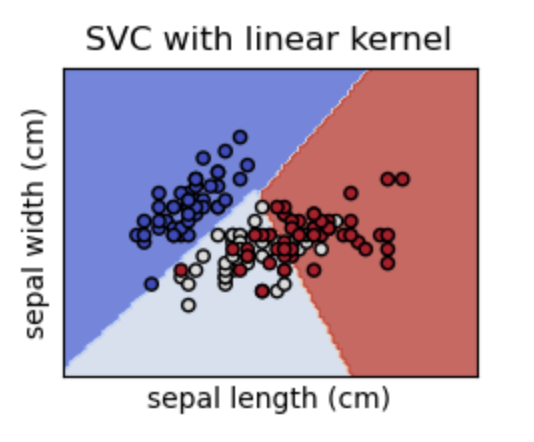
\includegraphics[width=0.35\textwidth]{./figures/svm_classical_example.png} 
    \caption{An Example SVM classifying data on the Iris dataset.}\label{fig:svm-classical}
\end{figure}
%\vspace{.15in}
%\newpage

Now that the stage is set from classical machine learning classification, it is time to dive into how a Variational
 Quantum Classifier works.


\section{Parameterized Quantum Circuits}\label{vqcircuits}

An essential part of many Quantum Machine Learning algorithms are Parameterized Quantum Circuits (PQCs). These are quantum Circuits
with some fixed gates like controlled NOTs (CNOT) and adjustable gates like Qubit Rotations. These circuits are good candidates
for demonstrating quantum advantage on near-term quantum devices because they can be optimized while taking into consideration gate
and other environmental noise \cite{Benedetti_2019}. Figure \ref{fig:pqc-dummy} 
below is an example of a simple parameterized circuit that takes a single parameter $\theta$ and then entangles $q_0$ and $q_1$


\begin{figure}[!h]
    \centering
    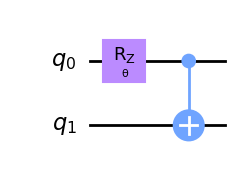
\includegraphics[width=0.3\textwidth]{./figures/pqc_example.png} 
    \caption{An Example Parameterized Quantum Circuit with Z Rotation with parameter $\theta $ and a single CNOT gate. 
    $\cite{qiskitPQC}$ }\label{fig:pqc-dummy}
\end{figure}

Since all gates used in a Quantum Circuit must be unitary, it is possible to describe a parameterized circuit as unitary operation 
on $n$ qubits, $U_\theta$, acting on some initial state $\ket{\phi_0}$, often set to $\ket{0}^{\otimes n}$~\cite{qiskitPQC}.
This leads to the resulting quantum state of the parameterized circuit: $\ket{\phi_\theta} = U_\theta\ket{\phi_0}$~\cite{qiskitPQC}.

When using PQCs for machine learning algorithms, it is important that the circuit be as generalized as possible. Researchers recently
proposed two measures to differentiate between different PQCs: expressibility and entangling capacity \cite{Sim_2019}.

\begin{itemize}
    \item \textit{Expressibility:} The coverage of the Hilbert space by a circuit. Circuits with high expressibility can 
    represent more unitaries. This can be quantified by the deviation from a uniform distribution \cite{Sim_2019} 
    See Figure \ref{fig:expressibility}

    \item \textit{Entangling Capacity:} Entanglement is a key resource in quantum computing. Meyer-Wallach defined a metric for how
    entangled a state is, with 0 being unentangled and 1 being maximally entangled (i.e. a Bell State) \cite{brennen2003observable}.
    Sim and others defined Entangling Capacity as the average Meyer-Wallach measure. See Figure \ref{fig:entangling-cap}
\end{itemize}

It has been shown that there is a strong correlation between expressibility and classification accuracy when using a Variational
Quantum Classifier \cite{hubregtsen2020evaluation}. Another consideration for selecting a PQC for a machine learning model is hardware
efficiency. To have any real impact in the near-term quantum computing era, the circuit depth is very important and directly impacts
the accuracy of many classifiers.
\begin{figure}[!h]
    \centering
    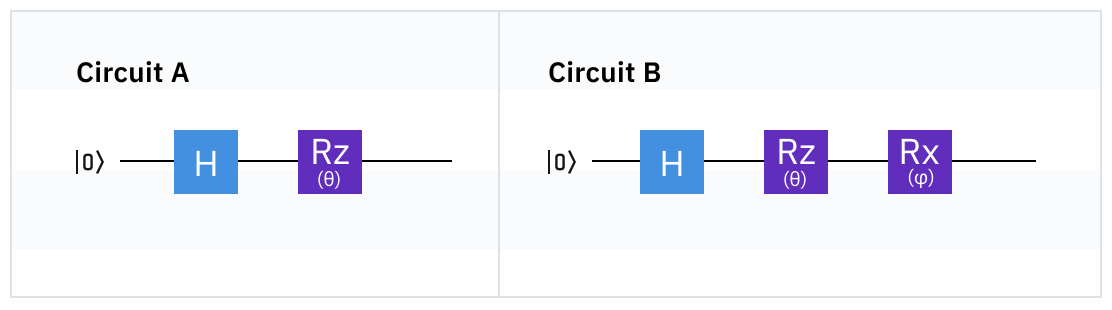
\includegraphics[width=0.6\textwidth]{./figures/Expressibility.png} 
    \caption{Example PQCs with different expressibility. Circuit A is low, while Circuit B is high. This means 
    that Circuit A can explore fewer states than Circuit B.~$\cite{qiskitPQC}$ }
    \label{fig:expressibility}
\end{figure}

\begin{figure}[!h]
    \centering
    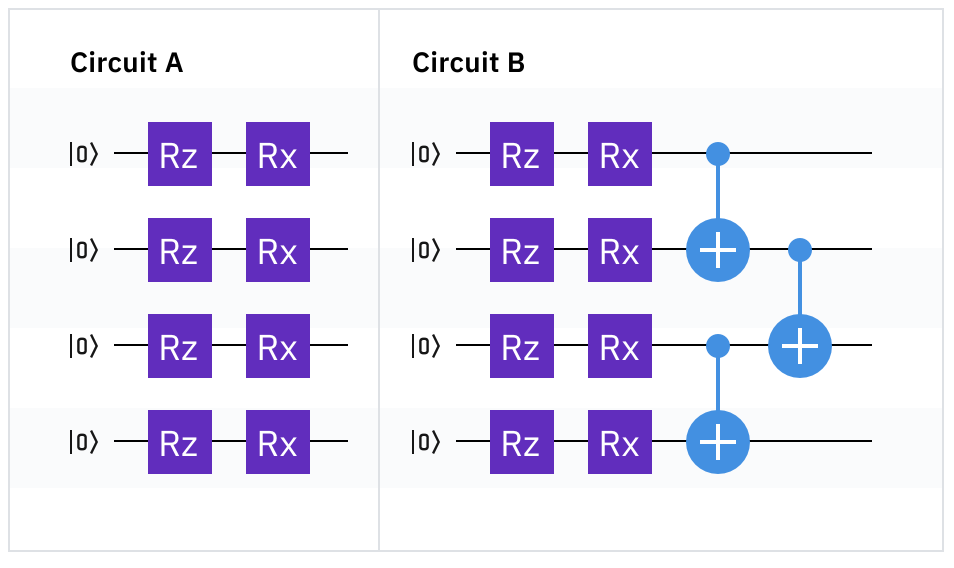
\includegraphics[width=0.50\textwidth]{./figures/Entangling-Capacity.png} 
    \caption{Example PQCs with different entangling capacity. Circuit A is low, while Circuit B is high. This means 
    that Circuit A is more limited in generating certain entangled states.~$\cite{qiskitPQC}$ }
    \label{fig:entangling-cap}
\end{figure}

PQCs are used mainly for two things in QML: \textit{encoding data} (where parameters are the input data) and as a 
\textit{Quantum Model}
where parameters are optimized in the training process.

\section{Data Encoding}\label{embedding}

In a Variational Quantum Classifier, it is important to have a way to map input data into a quantum circuit. This is typically done
with a PQC. Data Encoding is also referred to as data embedding, quantum embedding, or quantum reference state, 
where classical data is mapped into a quantum circuit using a quantum feature map. The goal is to take classical data $x$ 
and map into $\ket{\psi_x}$ using a set of gate parameters~\cite{SCHULD_2019_BOOK}. Some simple data embeddings are shown below. 
The \textit{ZZ Feature Map} is what used in this implementation of a VQC, shown later.

\subsection*{Basis Embedding}

Basis embedding maps each input with a computational basis state of a qubit system, hence the classical data must be 
able to be represented in binary strings. An entire dataset could be represented by the following equation assuming
 $D$ is a dataset with $x_n$: \cite{pennylaneQE}

 \[
    \ket{D} = \frac{1}{\sqrt{M}}\sum_{m=1}^{M}\ket{x^{(m)}}
 \]

Basis embedding is a good option for discrete data represented as binary or integers~\cite{pennylaneBLOG}.

\subsection*{Amplitude Embedding}

Amplitude Encoding is similar to basis encoding but instead of each input receiving its own computational basis, data is encoded into
the amplitudes of a quantum state. It requires the classical dataset to normalized so that each quantum state is valid. This embedding
can represent a normalized classical $N$-dimensional data point $x$ by the amplitudes of a $n$-qubit state $\ket{\psi_x}$ as:~\cite{pennylaneQE}

\[
    \ket{\psi_i} = \sum_{i=1}^{2^{n}}x_i\ket{i}
\]

Amplitude embedding is superb for modelling complex continuous data represented by complex values~\cite{pennylaneBLOG}.

\subsection*{Angle Embedding}
A simple encoding is also the angle embedding because it is simply a rotation along one of the axis of Rotation of the Bloch sphere. 
The following mapping demonstrates how encode data into a single qubit:

\[
    x \mapsto R_{k}(x)|0\rangle = e^{-i x\sigma_{k}/2}|0\rangle,    
\]

Angle embedding is great for continuous floating point data; however angle embedding typically leads to higher cost for optimization and construction \cite{pennylaneBLOG}.

\subsection*{ZZ Feature Map}\label{zzfeaturemapsection}

Each of the above techniques can be combined to create more complicated and higher order embeddings. These embeddings can also come with Hadamard gates interleaved
with entangling blocks. 
Researchers have found that a specific PQC known as \textit{ZZFeatureMap} is very effective on near-term hardware~\cite{Havl_ek_2019}. Below in Figure \ref{fig:ZZFeatureMap2}, two data points
are encoded into a quantum circuit. To expand to more data points, simply perform the Pauli Rotation with the next qubit and entangle with other qubits. 
Figure \ref{fig:ZZFeatureMap3} shows the expansion of this circuit to 3 qubits. This is the circuit that will be used later in the simulation of the VQC.

Now that the input data has been encoded into a quantum circuit using one of the above techniques, it is time to implement a quantum model.

\begin{figure}[!h]
    \centering
    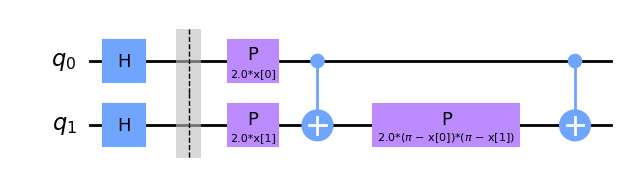
\includegraphics[width=0.8\textwidth]{./figures/two_qubit_feature_map.png} 
    \caption{Example of 2 data points $x_0$ and $x_1$ encoded into a ZZFeatureMap circuit using Qiskit}
    \label{fig:ZZFeatureMap2}
\end{figure}

\begin{figure}[!h]
    \centering
    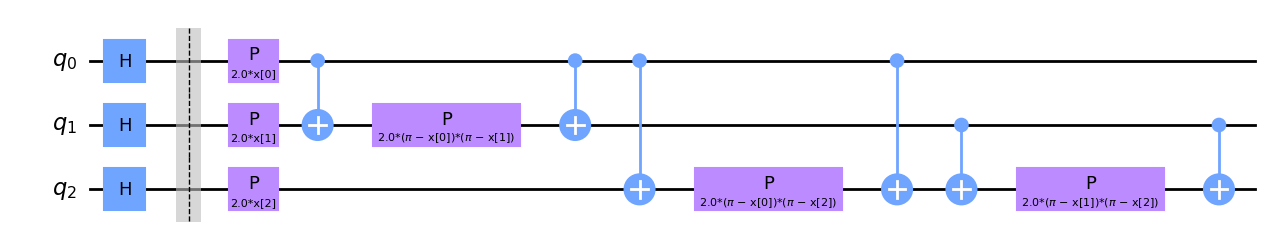
\includegraphics[width=1\textwidth]{./figures/three_qubit_feature_map.png} 
    \caption{Example of 3 data points $x_0$, $x_1$, and $x_2$ encoded into a ZZFeatureMap circuit using Qiskit}
    \label{fig:ZZFeatureMap3}
\end{figure}



\section{Quantum Model}\label{Quantum Model}

A quantum model is simply a specific parameterized circuit that can be optimized to increase accuracy. In the above section \ref{vqcircuits}, these circuits are explained in 
detail. In this section, Heuristics, trade-offs and examples will be shown. 

IBM researchers outline three trade-offs to consider when choosing a specific quantum model, and of course there is always a trade-off between speed and quality. More parameters
within the circuit is likely to become more accurate, but will take longer to run~\cite{ibmansatz}.

\begin{enumerate}
    \item \textbf{Speed:} Limiting the search space decreases the time it takes to run the algorithm (recall previous discussion of "expressibility") 
    \item \textbf{Accuracy:} Limiting the search space risks excluding the correct solution, leading to suboptimal results.
    \item \textbf{Noise:} Deep Circuits are impacted by noise heavily.
\end{enumerate}

Let's dive into some examples including N-Local Circuits, Two-Local, Real Amplitudes, and Efficient SU(2). For each example, the quantum circuit will be shown along with a brief
description.

\subsection*{N-Local Circuits}

N-Local Circuits (Figure~\ref{fig:nlocal}) are the most used heuristic models used and all the following circuits are derived from N-Local Circuits.
These circuits are great for quantum models because they have the best of all worlds when it comes to an efficient implementation while capturing the most important
correlations. The N represents the number of layers of rotation gates~\cite{ibmansatz}.

\begin{figure}[!h]
    \centering
    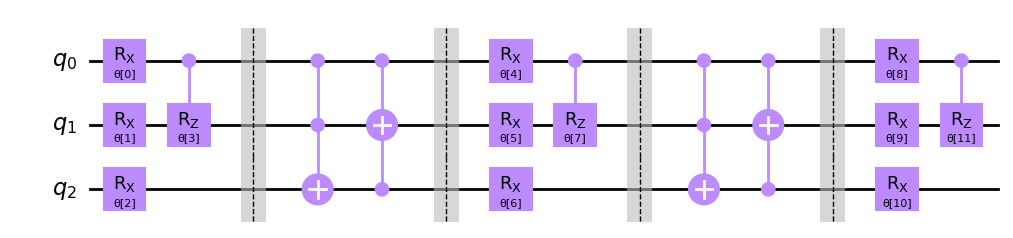
\includegraphics[width=1\textwidth]{./figures/nlocal.png} 
    \caption{Example of 3 Qubit NLocal circuit using Qiskit}
    \label{fig:nlocal}
\end{figure}

\subsection*{Two-Local Circuits}

Two Local Circuits (Figure~\ref{fig:2local}) are specific instance of N-Local Circuits where N is set to 2. This circuit consists of a single-qubit rotations and 2-qubit entanglement gates.
The types of rotations can be interchanged between $R_x$, $R_y$ and $R_z$, as well as the number of repetitions of this circuit~\cite{ibmansatz}.

\begin{figure}[!h]
    \centering
    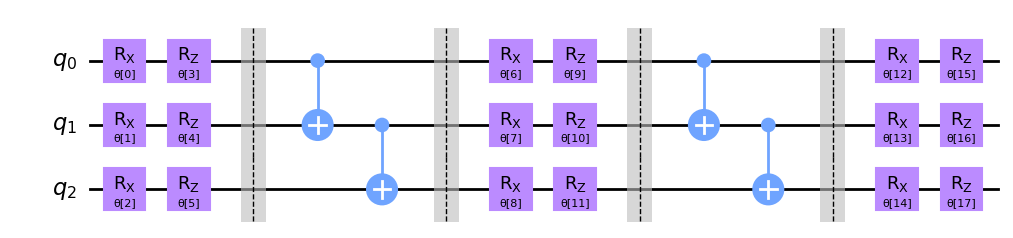
\includegraphics[width=1\textwidth]{./figures/2local.png} 
    \caption{Example of 3 qubit TwoLocal circuit using Qiskit}
    \label{fig:2local}
\end{figure}


\subsection*{Real Amplitudes}

Real Amplitudes (Figure~\ref{fig:realamplitudes}) is a specific instance of a Two-Local Circuit that has been used in chemistry applications alongside classification problems. Since all the amplitudes are real,
there is no complex parts. The circuit specifically uses $Y$ rotations and $CX$ entanglements~\cite{ibmansatz}.

\begin{figure}[!h]
    \centering
    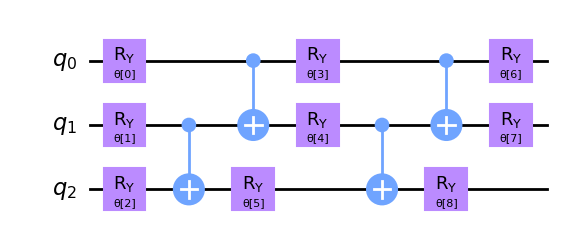
\includegraphics[width=0.75\textwidth]{./figures/realamplitudes.png} 
    \caption{Example of 3 qubit Real Amplitudes Circuit using Qiskit}
    \label{fig:realamplitudes}
\end{figure}

\subsection*{Efficient SU(2)}

Efficient SU(2) (Figure~\ref{fig:efficientsu2}) is also a specific version of a Two-Local circuit that uses $SU(2)$ and $CX$ entanglement, where $SU(2)$ is a special unitary group of degree 2 such as a Pauli
Rotation. This is a well known quantum model for machine learning on near-term devices because it has high expressibility and is very efficient on hardware~\cite{ibmansatz}.

\begin{figure}[!h]
    \centering
    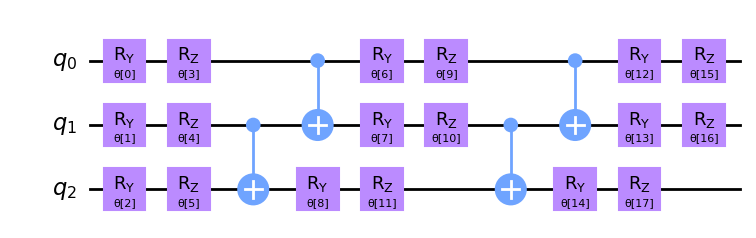
\includegraphics[width=1\textwidth]{./figures/efficientsu2.png} 
    \caption{Example of 3 qubit EfficientSU2 circuit with 2 repetitions using Qiskit}
    \label{fig:efficientsu2}
\end{figure}

The last three of these quantum models were used as the quantum model within the simulated VQC shown later. 

\section{Optimization and Prediction}\label{train}

This research isn't focused on the optimization and training process of these circuits. Briefly, it is notable that classical optimization algorithms can be used to tune the
parameterized quantum circuits. Techniques like gradient descent get generalized into a more efficient version using the Parameter Shift Rule~\cite{crooks2019gradients}.

Prediction and label assignment comes from probabilistic simulation of many shots of these circuits. Specifically, the predicted class comes as the computational state with
the highest probability. It is possible to define other functions to predict a class, but all of these methods rely on performing a measurement in the computational basis.

\section{Simulation}\label{sim}

Now, let's get into the fun part of investigating these Variational Quantum Classifiers.

\subsection*{Starting Point and Setup}

This research stems off of educational material from Qiskit~\cite{qiskit_sim}. The major changes from the initial tutorial code include the expansion to other datasets aside 
from the Iris Dataset as well as experimentation with different Ansatz Functions. The libraries used in this Python simulation are Qiskit and sklearn. 
Qiskit is meant for quantum programming while sklearn implements many classical
machine learning functions.

\subsection*{Datasets}

Three datasets were used for performance evaluation~\cite{sklearndata}. These are classic machine learning datasets: Iris, Wine, and Digits. For this effort, condensed versions were used to decrease 
computation time. Important notes about the datasets are found below:

\begin{itemize}
    \item \textbf{Iris:} 150 samples, 4 Features, 3 Classes, Numeric Data about sepal length, sepal width, petal length, and petal width.
    \item \textbf{Wine:} 178 samples, 13 Features, 3 Classes, Numeric Data about different wine attributes.
    \item \textbf{Digits:} 1797 samples, 17 Features, 10 Classes, Images of Handwritten digits 8$\times$8 values of 0-16 integers.
\end{itemize}

\subsection*{Implementation}
This section will detail the steps taken to implement the Variational Quantum Classifier. The full code will be attached with submission.

\begin{enumerate}
    \item Load the Data using `sklearn' functions.
    \item Train a Classical Machine Learning Model. In this research, a basic SVM was used with default parameters for comparison.
    \item Train a Quantum Machine Learning Model. 
    \begin{enumerate}
        \item Determine number of features from input data
        \item Select a feature map. In this case, ZZFeatureMap was used (discussed above \ref{zzfeaturemapsection})
        \item Select a quantum model or Ansatz. 3 quantum models were compared (TwoLocal, RealAmplitudes, and EfficientSU2)
        \item Select optimization and simulator functions. (This was not the focus off the research, so a default was chosen `COBYLA' and the Qiskit `Sampler' primitive )
        \item Train the model using `sklearn' ``fit()'' function 
        \item Evaluate the model using `sklearn' ``score()'' function 
    \end{enumerate}
\end{enumerate}

\subsection*{Results}

Above is the basic implementation steps that were taken in conducting this computer simulation. The following tables~\ref{fig:results} show the results on each of the datasets. One thing that 
was examined was the use a classical machine learning technique for dimensionality reduction known as Principal Component Analysis (PCA). 
This reduced the input features to the VQC significantly and allowed the simulation to run much quicker and sometimes increased the accuracy.

\begin{figure}[!ht]
    \centering
    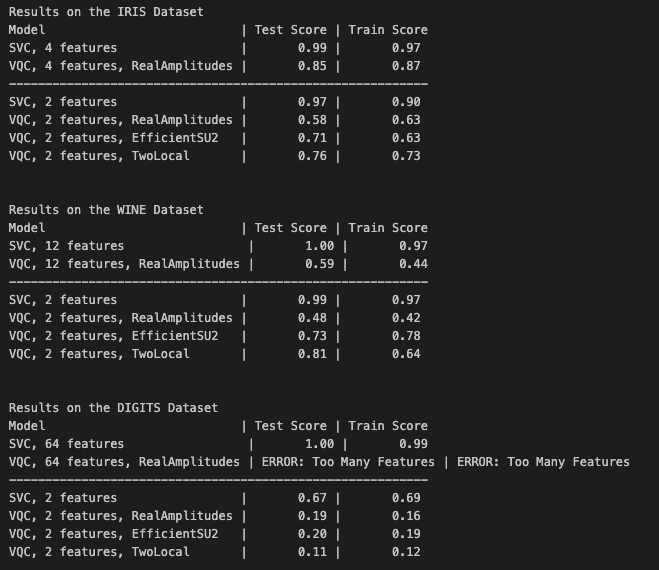
\includegraphics[width=1\textwidth]{./figures/results.png} 
    \caption{Screenshot of results for each of the three datasets}
    \label{fig:results}
\end{figure}

It can be seen that the TwoLocal Ansatz implementation seemed to have good results on the Wine and Iris datasets. The Digits dataset seemed 
to have poor performance overall and part of that is because of how the image dataset is encoded into the circuit. 

\newpage
\section{Challenges and Future Work}

Overall, the performance of this Variational Quantum Classifier is not superior to classical machine learning, and one of the main reasons is lack of training time. If more 
training cycles were used and more data was available, the accuracy would be improved. Another challenge is that the 64 features that were inputted
when the `digits' dataset was used caused the VQC to not compile using the IBM Sampler. 
 Future work would include investigation in better optimization algorithm that are 
\textit{``Quantum Aware''}. 

In conclusion, Variational Quantum Classifiers are an exciting field of research in Quantum Machine Learning as they can be implemented on near-term quantum computers to provide
valuables insights in the world today.

\newpage

\bibliographystyle{plain} % We choose the "plain" reference style
\bibliography{refs} % Entries are in the refs.bib file


\end{document}
